\documentclass{article}
% \VignettePackage{dapc}
% \VignetteIndexEntry{An introduction to Discriminant Analysis of Principal Components (DAPC)}

\usepackage{graphicx}
\usepackage[colorlinks=true,urlcolor=blue]{hyperref}
\usepackage{array}
\usepackage{color}

\usepackage[utf8]{inputenc} % for UTF-8/single quotes from sQuote()


% for bold symbols in mathmode
\usepackage{bm}

\newcommand{\R}{\mathbb{R}}
\newcommand{\beq}{\begin{equation}}
\newcommand{\eeq}{\end{equation}}
\newcommand{\m}[1]{\mathbf{#1}}



\newcommand{\code}[1]{{{\tt #1}}}
\title{A tutorial for Discriminant Analysis of Principal Components (DAPC) using \textit{adegenet} 1.3-0}
\author{Thibaut Jombart}
\date{\today}




\sloppy
\hyphenpenalty 10000


\usepackage{Sweave}
\begin{document}





\definecolor{Soutput}{rgb}{0,0,0.56}
\definecolor{Sinput}{rgb}{0.56,0,0}
\DefineVerbatimEnvironment{Sinput}{Verbatim}
{formatcom={\color{Sinput}},fontsize=\footnotesize, baselinestretch=0.75}
\DefineVerbatimEnvironment{Soutput}{Verbatim}
{formatcom={\color{Soutput}},fontsize=\footnotesize, baselinestretch=0.75}

\color{black}

\maketitle

\begin{abstract}
  This vignette provides a tutorial for applying the Discriminant Analysis of Principal Components
  (DAPC \cite{tjart19}) using the \textit{adegenet} package \cite{tjart05} for the R software
  \cite{np145}. This methods aims to identify and describe genetic clusters, although it can in fact
  be applied to any quantitative data. We illustrate how to use \code{find.clusters} to identify
  clusters, and \code{dapc} to describe the relationships between these clusters. More advanced
  topics are then introduced, such as advanced graphics, assessing the stability of DAPC results and
  using supplementary individuals.
\end{abstract}


\newpage
\tableofcontents


\newpage
%%%%%%%%%%%%%%%%
%%%%%%%%%%%%%%%%
\section{Introduction}
%%%%%%%%%%%%%%%%
%%%%%%%%%%%%%%%%


Investigating genetic diversity using multivariate approaches relies on finding synthetic variables
built as linear combinations of alleles (i.e. $\mbox{new-variable} = a_1 \mbox{allele}_1 + a_2 \mbox{allele}_2 + ... $
where $a_1$, $a_2$ etc. are real coefficients)
and which reflect as well as possible the genetic variation amongst the studied individuals.
However, most of the time we are not only interested in the diversity amongst individuals, but
also and possibly more in the diversity between groups of individuals.
Typically, one will be analysing individual data to identify populations, or more largely genetic
clusters, and then describe these clusters.

A problem occuring in traditional methods is they usually focus on the entire genetic variation.
Genetic variability can be decomposed using a standard multivariate ANOVA model as:
$$
\mbox{total variance} = \mbox{(variance between groups)} + \mbox{(variance within groups)}
$$
or more simply, denoting $\m{X}$ the data matrix:
$$
VAR(\m{X}) = B(\m{X}) + W(\m{X})
$$

Usual approaches such as Principal Component Analysis (PCA) or Principal Coordinates
Analysis (PCoA / MDS) focus on $VAR(\m{X})$. That is, they only describe the global diversity,
possibly overlooking differences between groups. On the contrary, DAPC optimizes $B(\m{X})$ while
minimizing $W(\m{X})$: it seeks synthetic variables, the \textit{discriminant functions}, which show
differences between groups as best as possible while minimizing variation within clusters.










%%%%%%%%%%%%%%%%
%%%%%%%%%%%%%%%%
\section{Identifying clusters using \code{find.clusters}}
%%%%%%%%%%%%%%%%
%%%%%%%%%%%%%%%%

%%%%%%%%%%%%%%%%
\subsection{Rationale}
%%%%%%%%%%%%%%%%
DAPC in itself requires prior groups to be defined. However, groups are often unknown or uncertain,
and there is a need for identifying genetic clusters before describing them. This can be achieved
using $k$-means, a clustering algorithm which finds a given (say, $k$) of groups maximizing the variation between
groups, $B(\m{X})$. To identify the optimal number of clusters, $k$-means is run sequentially with
increasing values of $k$, and different clustering solutions are compared using Bayesian Information
Criterion (BIC). Ideally, the optimal clustering solution should correspond to the lowest BIC. In
practice, the 'best' BIC is often indicated by an elbow in the curve of BIC values as a function of
$k$.

While $k$-means could be performed on the raw data, we prefer running the algorithm after
transforming the data using PCA. This transformation has the major advantage of reducing the
number of variables so as to speed up the clustering algorithm. Note this does not imply a necessary
loss of information since all the principal components (PCs) can be retained, and therefore all the variation in the original data.
However in practice, a reduced number of PCs is often sufficient to identify the existing clusters,
while making the analysis essentially instantaneous.


%%%%%%%%%%%%%%%%
\subsection{In practice}
%%%%%%%%%%%%%%%%

Identification of the clusters is achieved by \code{find.clusters}. This function first transforms
the data using PCA, asking the user to specify the number of retained PCs interactively unless the
argument \code{n.pca} is provided. Then, it runs $k$-means algorithm (function \code{kmeans} from
the \textit{stats} package) with increasing values of $k$, unless the argument  \code{n.clust} is
provided, and computes associated summary statistics (by default, BIC).
See \code{?find.clusters} for other arguments.

\code{find.clusters} is a generic function with methods for \texttt{data.frame}, objects with
the class \texttt{genind} (usual genetic markers) and \texttt{genlight} (genome-wide SNP data).
Here, we illustrate its use using a toy dataset simulated in \cite{tjart19}, \texttt{dapcIllus}:
\begin{Schunk}
\begin{Sinput}
> library(adegenet)
> data(dapcIllus)
> class(dapcIllus)
\end{Sinput}
\begin{Soutput}
[1] "list"
\end{Soutput}
\begin{Sinput}
> names(dapcIllus)
\end{Sinput}
\begin{Soutput}
[1] "a" "b" "c" "d"
\end{Soutput}
\end{Schunk}

\texttt{dapcIllus} is a list containing four datasets; we shall only use the first one:
\begin{Schunk}
\begin{Sinput}
> x <- dapcIllus$a
> x
\end{Sinput}
\begin{Soutput}
   #####################
   ### Genind object ### 
   #####################
- genotypes of individuals - 

S4 class:  genind
@call: read.fstat(file = file, missing = missing, quiet = quiet)

@tab:  600 x 140 matrix of genotypes

@ind.names: vector of  600 individual names
@loc.names: vector of  30 locus names
@loc.nall: number of alleles per locus
@loc.fac: locus factor for the  140 columns of @tab
@all.names: list of  30 components yielding allele names for each locus
@ploidy:  2
@type:  codom

Optionnal contents: 
@pop:  factor giving the population of each individual
@pop.names:  factor giving the population of each individual

@other: - empty -
\end{Soutput}
\end{Schunk}
\texttt{x} is a dataset of 600 individuals simulated under an island model (6 islands) for 30 microsatellite markers.
We use \code{find.clusters} to identify clusters, although true clusters are, in this case, known
(and accessible using \texttt{pop(x)}).
We specify that we want to evaluate up to $k=40$ groups (\texttt{max.n.clust=40}):
\begin{Schunk}
\begin{Sinput}
> grp <- find.clusters(x, max.n.clust = 40)
\end{Sinput}
\end{Schunk}

\begin{center}
  \includegraphics[width=.7\textwidth]{figs/findclust-pca.pdf}
\end{center}

\noindent
The function displays a graph of cumulated variance explained by the eigenvalues of the PCA.
Apart from computational time, there is no reason for keeping a small number of components; here, we
keep all the information, specifying to retain 200 PCs (there are actually less PCs ---around 110---, so all of them
are kept).

Then, the function displays a graph of BIC values for increasing values of $k$:
\begin{center}
  \includegraphics[width=.7\textwidth]{figs/findclust-bic.pdf}
\end{center}

\noindent This graph shows a clear decrease of BIC until $k=6$ clusters, after which BIC increases.
In this case, the elbow in the curve also matches the smallest BIC, and clearly indicates 6 clusters
should be retained. In practice, the choice is often trickier to make for empirical dataset.
\\

The output of \texttt{find.clusters} is a list:
\begin{Schunk}
\begin{Sinput}
> names(grp)
\end{Sinput}
\begin{Soutput}
[1] "Kstat" "stat"  "grp"   "size" 
\end{Soutput}
\begin{Sinput}
> head(grp$Kstat, 8)
\end{Sinput}
\begin{Soutput}
NULL
\end{Soutput}
\begin{Sinput}
> grp$stat
\end{Sinput}
\begin{Soutput}
NULL
\end{Soutput}
\begin{Sinput}
> head(grp$grp, 10)
\end{Sinput}
\begin{Soutput}
001 002 003 004 005 006 007 008 009 010 
  2   2   2   6   2   2   2   2   2   2 
Levels: 1 2 3 4 5 6
\end{Soutput}
\begin{Sinput}
> grp$size
\end{Sinput}
\begin{Soutput}
[1]  99  98  99 102  97 105
\end{Soutput}
\end{Schunk}

The components are respectively the chosen summary statistics (here, BIC) for different values of
$k$ (slot \texttt{Kstat}), the selected number of clusters and the associated BIC (slot
\texttt{stat}), the group memberships (slot \texttt{grp}) and the group sizes (slot \texttt{size}).
Here, since we know the actual groups, we can check how well they have been retrieved by the procedure.
Actual groups are accessed using \texttt{pop}:
\begin{Schunk}
\begin{Sinput}
> table(pop(x), grp$grp)
\end{Sinput}
\begin{Soutput}
      1   2   3   4   5   6
  1   0  97   0   0   0   3
  2  99   0   0   0   0   1
  3   0   0  98   0   2   0
  4   0   0   0 100   0   0
  5   0   1   0   2  95   2
  6   0   0   1   0   0  99
\end{Soutput}
\begin{Sinput}
> table.value(table(pop(x), grp$grp), col.lab = paste("inf", 1:6), 
+     row.lab = paste("ori", 1:6))
\end{Sinput}
\end{Schunk}
\includegraphics{figs/dapc-006}

\noindent
Rows correspond to actual groups ("ori''), while columns correspond to inferred groups ("inf'').
Here, we can see that original groups have nearly been perfectly identified by the method.


%%%%%%%%%%%%%%%%
\subsection{How many clusters are there really in the data?}
%%%%%%%%%%%%%%%%

Although the most frequently asked when trying to find clusters in genetic data, this question is
equally often meaningless. Clustering algorithms help making a caricature of a complex reality,
which is most of the time far from following known population genetics models. Therefore, we are
rarely looking for actual panmictic populations from which the individuals have been drawn. Genetic
clusters can be biologically meaningful structures and reflect interesting biological processes, but
they are still models.

A slightly different but probably more relevant question would be: "How many clusters are useful to
describe the data?''. A fundamental point in this question is that clusters are merely tools used to
summarise and understand the data. There is no longer a "true $k$", but some values of $k$ are
better, more efficient summaries of the data than others.
For instance, in the following case:
\begin{center}
  \includegraphics[width=.7\textwidth]{figs/findclust-noclearcut.pdf}
\end{center}

\noindent , the concept of "true $k$" is fairly hypothetical. This does not mean that clutering
algorithms should necessarily be discarded, but surely the reality is more complex than a few
clear-cut, isolated populations. What the BIC decrease says is that 10-20 clusters would provide useful
summaries of the data. The actual number retained is merely a question of personnal taste.









%%%%%%%%%%%%%%%%
%%%%%%%%%%%%%%%%
\section{Describing clusters using \code{dapc}}
%%%%%%%%%%%%%%%%
%%%%%%%%%%%%%%%%


%%%%%%%%%%%%%%%%
\subsection{Rationale}
%%%%%%%%%%%%%%%%
DAPC aims to provide an efficient description of genetic clusters using a few synthetic variables.
These are constructed as linear combinations of the original variables (alleles) which have the
largest between-group variance and the smallest within-group variance. Coefficients of the alleles
used in the linear combination are called \textit{loadings}, while the synthetic variables are
themselves referred to as \textit{discriminant functions}.

Moreover, being based on the Discriminant Analysis, DAPC also provides membership probabilities of
each individual for the different groups based on the retained discriminant functions. While these
are different from the admixture coefficients of software like STRUCTURE, they can still be
interpreted as proximities of individuals to the different clusters. Membership
probabilities also provide indications of how clear-cut genetic clusters are. Loose clusters will
result in fairly flat distributions of membership probabilities of individuals across clusters,
pointing to possible admixture.

Lastly, using the allele loadings, it is possible to represent new individuals (which have not participated to the analysis)
onto the factorial planes, and derive membership probabilities as welll. Such individuals are
referred to as \textit{supplementary individuals}.



%%%%%%%%%%%%%%%%
\subsection{In practice}
%%%%%%%%%%%%%%%%

DAPC is implemented by the function \texttt{dapc}, which first transforms the data using PCA, and
then performs a Discriminant Analysis on the retained principal components. Like
\texttt{find.clusters}, \texttt{dapc} is a generic function with methods for \texttt{data.frame}, and objects with
the class \texttt{genind} (usual genetic markers) and \texttt{genlight} (genome wide SNP data).

We run the analysis on the previous toy dataset, using the inferred groups stored in \texttt{grp\$grp}:

\begin{Schunk}
\begin{Sinput}
> dapc1 <- dapc(x, grp$grp)
\end{Sinput}
\end{Schunk}

The method displays the same graph of cumulated variance as in \texttt{find.cluster}. However, unlike
$k$-means, DAPC can benefit from not using too many PCs. Indeed, retaining too many components with
respect to the number of individuals can lead to over-fitting and unstability in the membership
probabilities returned by the method (see section below about the stability of membership probabilities).

\begin{center}
  \includegraphics[width=.7\textwidth]{figs/findclust-pca.pdf}
\end{center}

\noindent The bottomline is therefore retaining a few PCs without sacrificing too much information.
Here, we can see that little information is gained by adding PCs after the first 40. We therefore
retain 40 PCs.

Then, the method displays a barplot of eigenvalues for the discriminant analysis, asking for a
number of discriminant functions to retain (unless argument \texttt{n.da} is provided).
\begin{center}
  \includegraphics[width=.7\textwidth]{figs/eigen-dapc.pdf}
\end{center}

For small number of clusters, all eigenvalues can be retained since all discriminant functions can
be examined without difficulty. Whenever more (say, tens of) clusters are analysed,
it is likely that the first few dimensions will carry more information than the others, and only
those can then be retained and interpreted.
\\

The object \texttt{dapc1} contains a lot of information:
\begin{Schunk}
\begin{Sinput}
> dapc1
\end{Sinput}
\begin{Soutput}
	#########################################
	# Discriminant Analysis of Principal Components #
	#########################################
class: dapc
$call: dapc.genind(x = x, pop = grp$grp, n.pca = 40, n.da = 100)

$n.pca: 40 first PCs of PCA used
$n.da: 5 discriminant functions saved
$var (proportion of conserved variance): 0.915

$eig (eigenvalues): 874.1 703.2 541.5 447.9 365.3  vector    length content                   
1 $eig      5      eigenvalues               
2 $grp      600    prior group assignment    
3 $prior    6      prior group probabilities 
4 $assign   600    posterior group assignment
5 $pca.cent 140    centring vector of PCA    
6 $pca.norm 140    scaling vector of PCA     
7 $pca.eig  0      eigenvalues of PCA        

  data.frame    nrow ncol content                                          
1 $tab          600  40   retained PCs of PCA                              
2 $means        6    40   group means                                      
3 $loadings     40   5    loadings of variables                            
4 $ind.coord    600  5    coordinates of individuals (principal components)
5 $grp.coord    6    5    coordinates of groups                            
6 $posterior    600  6    posterior membership probabilities               
7 $pca.loadings 140  40   PCA loadings of original variables               
8 $var.contr    140  5    contribution of original variables               
\end{Soutput}
\end{Schunk}

For details about this content, please read the documentation (\texttt{?dapc}).
Essentially, the slots \texttt{ind.coord} and \texttt{grp.coord} contain the coordinates of the
individuals and of the groups used in scatterplots.
Contributions of the alleles to each discriminant function are stored in the slot \texttt{var.contr}.
Eigenvalues, corresponding to the ratio of the variance between groups over the variance within
group for each discriminant function, are stored in \texttt{eig}.
Basic scatterplots can be obtained using the function \texttt{scatterplot}:
\begin{Schunk}
\begin{Sinput}
> scatter(dapc1)
\end{Sinput}
\end{Schunk}
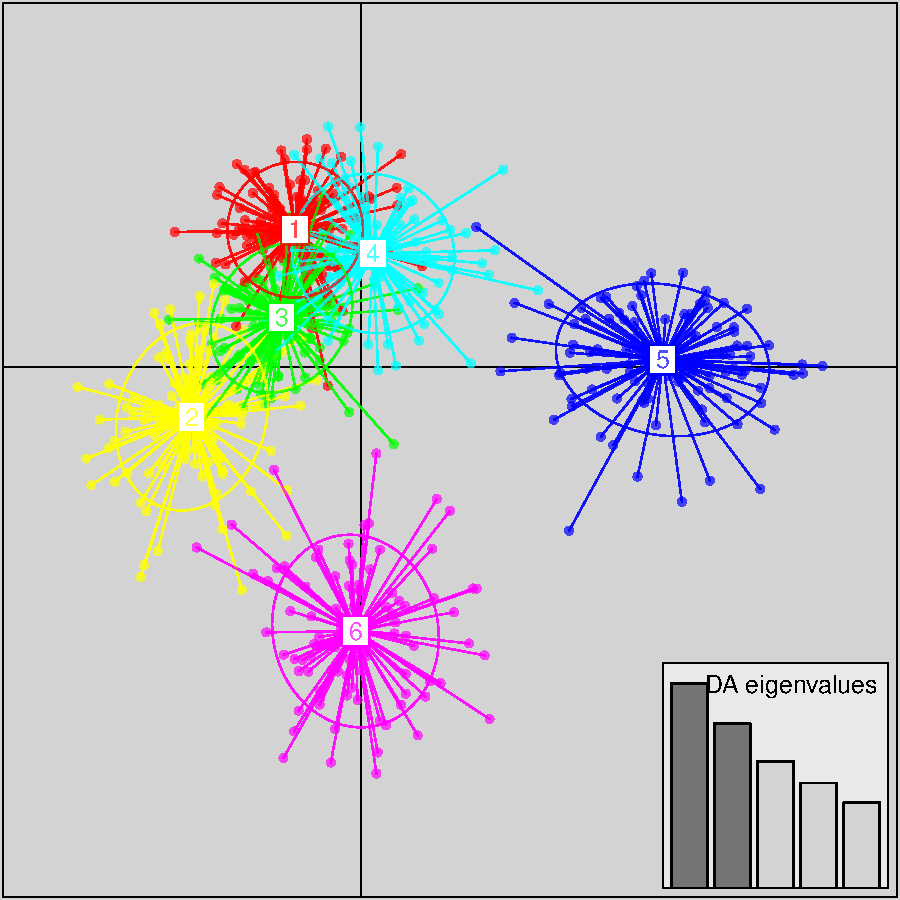
\includegraphics{figs/dapc-010}

\noindent The obtained graph represents the individuals as dots and the groups as inertia
ellipses. Eigenvalues of the analysis are displayed in inset. These graphs are fairly easy to
customize, as shown below.




%%%%%%%%%%%%%%%%
\subsection{Customizing DAPC scatterplots}
%%%%%%%%%%%%%%%%

DAPC scatterplots are the main result of DAPC. It is therefore essential to ensure that information
is displayed efficiently, and if possible to produce pretty figures.
Possibility are almost unlimited, and here we just illustrate a few possibilities offered by
\texttt{scatter}. Note that \texttt{scatter} is a generic function, with a dedicated method for
objects produced by \texttt{dapc}. Documentation of this function can be accessed by typing \texttt{?scatter.dapc}.

We illustrate some graphical possibilities trying to improve the display of the analysis presented
in the previous section.
While the default background (grey) allows to visualize rainbow colors (the default palette for the
groups) more easily, it is not so pretty and is probably better removed for publication purpose.
We also move the inset to a more appropriate place where it does not cover individuals, and use
different symbols for the groups.

\begin{Schunk}
\begin{Sinput}
> scatter(dapc1, posi.da = "bottomright", bg = "white", pch = 17:22)
\end{Sinput}
\end{Schunk}
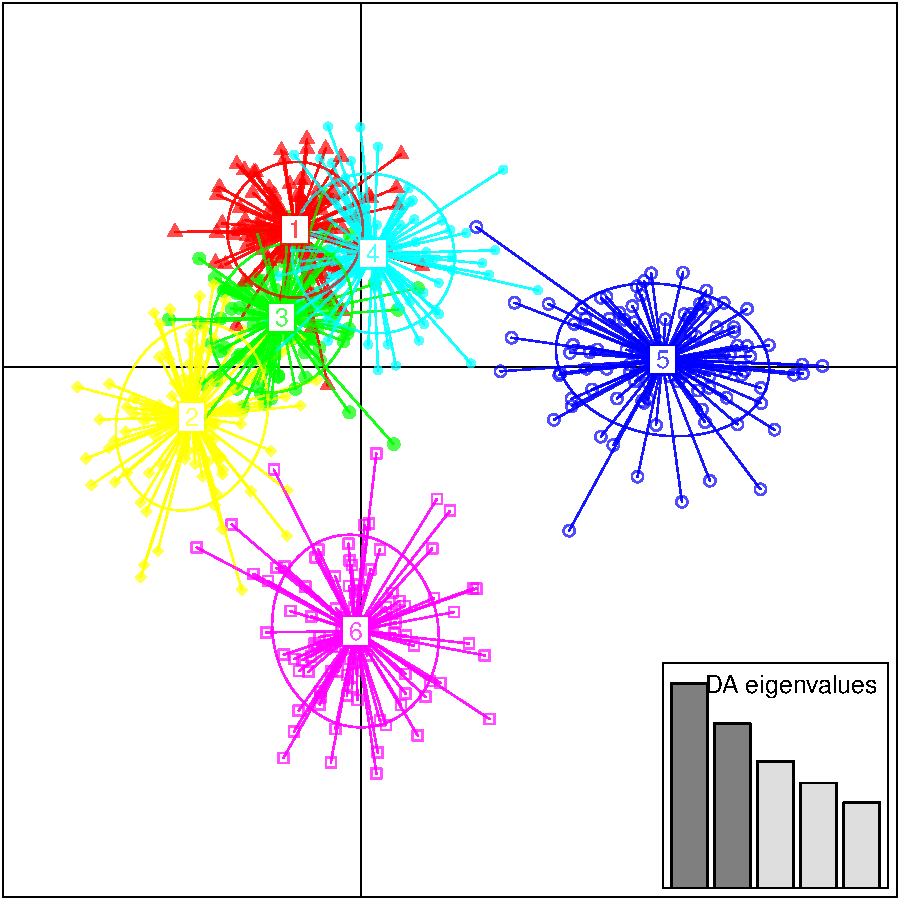
\includegraphics{figs/dapc-011}

\noindent This is still not entirely satisfying: we need to define other colors more visible over a white
background, and we can remove the segments linking the points to their ellipses:
\begin{Schunk}
\begin{Sinput}
> myCol <- c("darkblue", "purple", "green", "orange", "red", "blue")
> scatter(dapc1, posi.da = "bottomright", bg = "white", pch = 17:22, 
+     cstar = 0, col = myCol, scree.pca = TRUE, posi.pca = "bottomleft")
\end{Sinput}
\end{Schunk}
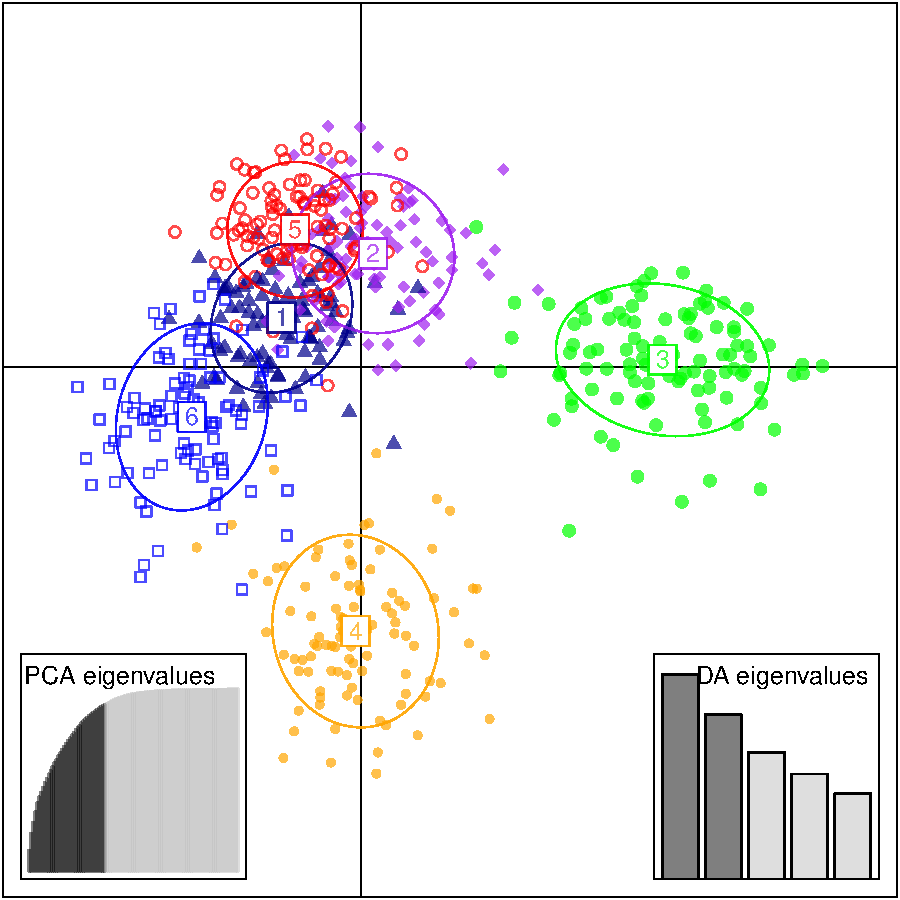
\includegraphics{figs/dapc-012}

\noindent Another possibility is remove the labels within the ellipses and add a legend to the
plot. We also use the same symbol for all individuals, but use bigger dots and transparent colours
to have a better feel for the density of individuals on the factorial plane.
\begin{Schunk}
\begin{Sinput}
> scatter(dapc1, scree.da = FALSE, bg = "white", pch = 20, cell = 0, 
+     cstar = 0, col = myCol, solid = 0.4, cex = 3, clab = 0, leg = TRUE, 
+     txt.leg = paste("Cluster", 1:6))
\end{Sinput}
\end{Schunk}
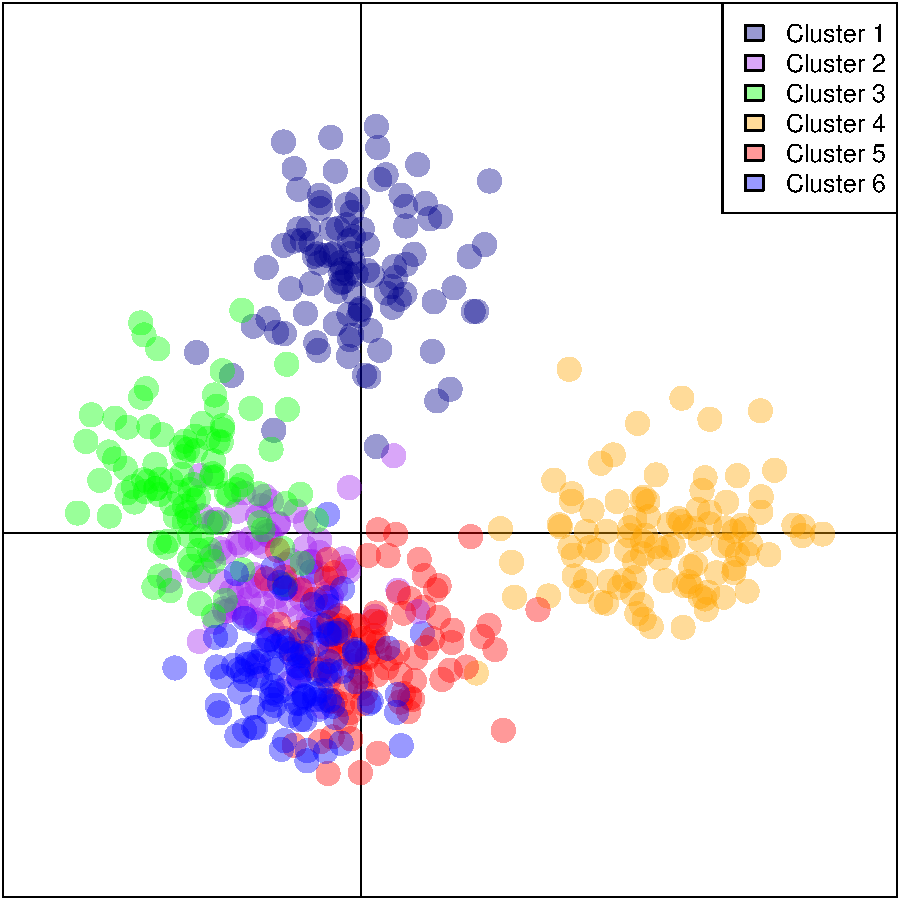
\includegraphics{figs/dapc-013}

We can also add a minimum spanning tree based on the (squared) distances between populations in the
entire space.
This allows one to bear in mind the actual proximities between populations inside the entire space, which are not always
well represented in susbsets of discriminant functions of lesser rank.
We also indicate the centre of each group with crosses.
Lastly, we remove the DAPC eigenvalues, not very useful in this case, and replace them manually by a graph of
PCA eigenvalues retained in dimension-reduction step (retained eigenvalues in black, similar to
using \texttt{scree.pca=TRUE}).
\begin{Schunk}
\begin{Sinput}
> scatter(dapc1, ratio.pca = 0.3, bg = "white", pch = 20, cell = 0, 
+     cstar = 0, col = myCol, solid = 0.4, cex = 3, clab = 0, mstree = TRUE, 
+     scree.da = FALSE, posi.pca = "bottomright", leg = TRUE, txt.leg = paste("Cluster", 
+         1:6))